\documentclass[11pt,a4paper]{article}
\usepackage[UTF8]{ctex}
\usepackage[margin=2.35cm]{geometry}
\usepackage{amsmath,amssymb,booktabs,tabularx,array,hyperref,tikz,graphicx,listings,xcolor}
\usetikzlibrary{positioning,calc}
\usepackage[backend=biber,style=gb7714-2015]{biblatex}
\addbibresource{references.bib}

\hypersetup{colorlinks=true,linkcolor=blue,citecolor=blue,urlcolor=blue}
\newcolumntype{Y}{>{\raggedright\arraybackslash}X}
\lstset{basicstyle=\ttfamily\footnotesize,breaklines=true,frame=single,columns=fullflexible,showstringspaces=false}
\title{\heiti 多模态大模型与智能体驱动的脑病跨尺度分析\\\large 以脑细胞外间隙（ECS）研究为例}
\author{\heiti 冉源潮}
\date{2026年7月}

\begin{document}
\maketitle

\begin{abstract}
脑细胞外间隙（ECS）由细胞外液、细胞外基质及其曲折微通道构成，参与离子稳态、神经活性物质扩散与代谢物清除。其微尺度结构难以被单一临床检查直接测量，因此脑病研究需要整合影像、病理、组学、时序生理信号和临床文本等异构证据。本文区分多模态大模型的联合表征能力与智能体的受约束工具编排能力，讨论二者在ECS相关脑病研究和临床辅助中的价值、局限及可验证实现路径。核心主张是：其价值不在于跨越尺度直接给出确定性诊断，而在于构建受物理规律与临床证据约束的假设生成与验证空间。为降低死后组织、动物实验与活体MRI之间的域偏移风险，框架将不确定性量化纳入跨尺度映射；面对真实临床中的缺失模态，智能体以预期信息增益而非模态完整性为目标，提出可由医生审核的补充检查建议。通过显式保留尺度差异、不确定性、证据来源和人类复核权限，该框架可为ECS相关机制研究与临床辅助提供可追溯的计算路径。
\end{abstract}

\noindent\textbf{关键词：}脑细胞外间隙；多模态学习；大语言模型；智能体；不确定性量化；人在回路

\tableofcontents
\clearpage

\section{引言}
ECS并非细胞之间的被动空隙，而是神经元、胶质细胞和血管相关细胞之间的动态传质空间。其体积分数$\alpha$、曲折度$\lambda$与有效扩散系数$D^*$常用于描述局部运输受限程度，经典近似为$D^*=D/\lambda^2$\cite{sykova2008,nicholson1998}。活脑超分辨成像提示，ECS在微尺度上具有显著空间异质性\cite{tonnesen2018}；不同物种、状态、测量方法及空间尺度下的参数不宜直接互换。

脑水肿和缺血可伴随细胞肿胀与细胞外体积改变；创伤、癫痫、神经退行性病变、肿瘤微环境及炎症也可能重塑细胞外基质或间质运输。上述关联是研究问题而非自动成立的因果链，仍需纵向影像、组织学与干预实验共同验证。脑脊液--间质液交换及类淋巴相关机制具有重要研究价值，但其路径和驱动因素仍存在方法学争议\cite{iliff2012,mestre2020}。

\section{概念与核心技术架构}
\subsection{大模型、多模态模型与智能体的边界}
大模型通过大规模预训练获得可迁移表征或生成能力；多模态模型进一步从影像、文本、结构化变量、波形或组学等输入学习联合表示；智能体则是在明确权限、工具与停止规则下，调用模型、数据库或分析软件完成多步骤任务的执行系统。三者不应混同：联合表示不能保证物理规律成立，工具调用也不能替代临床证据判断。

一个面向ECS的系统可由五层组成：（1）模态专属编码器，将MRI、病理切片、EEG/MEG、表格和文本转为表示；（2）以受试者、脑区、采集时点和协议为键的跨模态对齐与融合；（3）检索增强生成（RAG），使生成性说明链接至版本化文献与本地数据字典\cite{lewis2020}；（4）智能体编排质控、分割、统计、物理反演和报告工具，并保留调用日志；（5）人类复核、访问控制与不确定性呈现。ReAct等框架说明了推理--行动--观察的工具协作范式\cite{yao2023}，但医疗任务仍须限制工具权限与输出范围。

\subsection{生物医学优势与必要约束}
多模态方法可将影像的空间信息、病历文本的病程信息、实验记录的条件信息和组学的分子信息置于同一可查询框架；基础模型也可能降低小样本任务的标注需求\cite{moor2023}。但缺失模态、中心间扫描协议差异、选择偏倚、标签噪声和域迁移均可造成性能虚高。生成模型还可能产生无来源的幻觉，相关性模型不能据此宣称因果关系。临床部署前必须报告校准度、亚组表现、失败模式与外部验证结果，并满足隐私、伦理和全生命周期变更管理要求\cite{topol2019,fdaaiml2021}。

\section{阿尔茨海默病：ECS清除障碍的多模态闭环}
\subsection{从类淋巴交换到A$\beta$/Tau蓄积的可检验问题}
阿尔茨海默病（AD）为本文重点场景。脑脊液--间质液交换及血管周围通路可能参与可溶性代谢物清除；星形胶质细胞足突中AQP4的血管周围极化被提出为影响该过程的关键因素之一\cite{iliff2012,zeppenfeld2017}。人脑死后组织研究报告，AQP4定位改变与AD病理负荷相关\cite{zeppenfeld2017}；这提示血管周围微环境重塑--间质运输改变--A$\beta$/Tau负荷是值得检验的跨尺度假设，而非已由单一指标证实的因果序列。睡眠、衰老、血管危险因素和炎症均可能构成混杂或效应修饰因素，应在队列设计中预先记录和建模\cite{xie2013,mestre2020}。

具体而言，问题可表述为：在年龄、睡眠、血管危险因素和疾病阶段可比的个体中，宏观扩散代理、血管周围间隙表型、A$\beta$/Tau体液标志物与AQP4相关微观证据能否形成一致的可计算联合表型？若能，该表型能否预测纵向认知或病理标志物变化？该问题将类淋巴清除受损拆解为可测量、可反驳的子问题，并为动物模型干预提供分层假设和明确终点。

\subsection{AD多模态价值矩阵}
\begin{table}[htbp]\centering\small
\caption{以AD的ECS/类淋巴清除障碍为例的跨尺度证据矩阵\label{tab:ad}}
\begin{tabularx}{\linewidth}{p{2.5cm}Y Y Y}\toprule
证据层级 & 代表数据与可提取特征 & 与清除假设的关系 & 验证或解释边界\\\midrule
宏观影像 & T1/FLAIR的PVS表型；DWI/DTI中DTI-ALPS扩散代理；动态对比增强或灌注数据（如有） & 描述血管周围和水扩散的个体、纵向表型 & DTI-ALPS不是直接的类淋巴流量或ECS几何测量；需控制扫描协议\cite{taoka2021}\\
分子与临床 & CSF或血液A$\beta$、p-tau、总Tau；认知量表、睡眠和血管危险因素 & 提供病理负荷、病程与混杂因素的时序锚点 & 标志物变化不等同于某一清除通路的特异性改变\\
微观组织与空间组学 & AQP4极化、血管周围基底膜、A$\beta$沉积；空间转录组中的星形胶质细胞/血管周围细胞状态 & 提供宏观影像表型的组织学候选解释 & 多来自死后组织或动物；不能逐例直接外推至活体MRI\\
智能体产物 & 带来源的影像--分子--微观证据联合表型与待检验机制图 & 发现一致或矛盾证据，生成分层与随访假设 & 不是诊断标签；结论须由独立队列和干预研究检验\\\bottomrule
\end{tabularx}
\end{table}

例如，智能体可在DTI质控通过后提取DTI-ALPS等影像代理，链接同一受试者的A$\beta$/Tau时间序列、睡眠与血管危险因素；再从版本化知识库检索AQP4极化和血管周围基底膜的空间组学或病理证据。输出不应写成患者清除功能下降的确定性结论，而应是与清除受损假设一致的分子--影像联合表型，并列出替代解释、数据缺口和下一步验证方案。模型的价值在于将分散证据转化为可追溯的研究问题。

\section{ECS相关多模态数据及应用价值}
\begin{table}[htbp]\centering\small
\caption{多模态数据在ECS相关脑病研究中的任务、价值与验证要求\label{tab:data}}
\begin{tabularx}{\linewidth}{p{2.2cm}Y Y Y}\toprule
数据模态 & 可回答的问题（示例） & 科研或临床辅助价值 & 风险与验证方式\\\midrule
MRI：DWI/ADC、T1/T2、FLAIR、DTI、灌注 & 水扩散、结构损伤、血流与白质微结构的宏观代理 & 病灶定位、分层和纵向表型 & 不是ECS直接测量；需协议一致性、重复扫描和外部队列验证\\
CT、PET & 急性出血/水肿、代谢或受体相关信号 & 急诊信息互补、机制关联 & 辐射、时间不同步和非特异性；需临床金标准核对\\
EEG/MEG与生理波形 & 神经网络活动及其时间关系 & 癫痫等动态表型研究 & 伪迹和空间定位限制；需盲法事件标注\\
病理、动物实验、ECS动态示踪 & 细胞--基质边界及局部传质假设 & 机制验证与参数先验 & 与人体宏观影像存在尺度鸿沟；需独立重复与预注册\\
病历、检验、脑脊液、组学与文献 & 病程、炎症/代谢背景和候选通路 & 表型定义、假设生成和证据追溯 & 混杂、批次效应和隐私风险；需数据字典、去标识与审计\\\bottomrule
\end{tabularx}
\end{table}

MRI的DWI/ADC、DTI和DTI-ALPS等指标可提供水扩散或血管周围方向扩散的宏观代理，但不能表述为对ECS几何参数的直接测量\cite{taoka2021}。病理和活体示踪可补充微尺度信息，CSF/血液检测与组学可描述分子环境，病历与量表可锚定功能结局。合理融合应显式保留尺度、时间差和缺失状态，而不是把一种模态翻译为另一种模态。

在科研中，系统可筛选结构改变--运输表型--分子通路的关联模式，形成待验证假设。在临床中，系统可辅助汇总影像、病史和检验资料，提示低置信输入、缺失检查及与证据不一致之处；它不应取代放射科、神经科或病理医师的判断。

\section{可实现且可验证的技术路线}

\subsection{跨尺度对齐：从微观组织图到MRI体素}
病理切片或空间转录组的分辨率与MRI体素相差数个数量级，不能直接拼接后交由交叉注意力处理。可先建立\textbf{分层中间表示}：在同一脑区的组织学图像中分割血管、星形胶质细胞、细胞外基质和沉积物，构建细胞--血管--基质异质图；节点包含AQP4极化、基底膜/沉积负荷和局部转录特征，边表示空间邻接或血管周围关系。再以脑区、层级和解剖坐标为锚点，将细胞类型比例、图谱模块分数和连通性聚合为虚拟组织图谱。图神经网络可将微观图的节点信息映射为脑区级特征，并与MRI体素级表征以层级对比学习对齐\cite{kipf2017}。

跨尺度映射的主要风险不是网络容量不足，而是域偏移。死后组织的自溶、固定和切片形变，AD相关脑萎缩、动物与人脑的血管及胶质结构差异，均可改变形态学特征的含义。对无配对的活体MRI与死后/动物空间组学，模型至多学习群体级先验，必须显式标注非个体配对，不得生成虚构的患者级空间转录组。建议以贝叶斯分层推断输出映射后验分布，并以Dempster--Shafer证据理论区分支持、反对和无知质量\cite{shafer1976}；同时报告中心、物种、死后间隔和萎缩程度分层的域外不确定性。医疗深度学习中的UQ还应同时检验校准度、分布外检测和风险--覆盖率曲线，避免仅以置信分数代替可靠性\cite{gawlikowski2023}。若映射置信度低或证据冲突，应退回脑区级假设，或拒绝给出微观解释，而非以单一点估计掩盖系统性偏差。

\subsection{数据与建模}
首先预先定义病例/样本队列、纳入排除标准、目标任务、主要终点及数据使用权限。执行DICOM完整性检查、影像伪迹控制、病理染色批次校正、组学批次校正和缺失机制标记；训练、调参与测试集须按患者和中心严格隔离。模型可采用模态专属预训练编码器与交叉注意力融合，并以掩码训练提高缺失模态鲁棒性。输出应包括来源模态、置信区间或预测集合、适用域判断和不能回答的问题。

对示踪浓度$C$的研究性反演，可将扩散--对流--清除模型作为待检验约束：
\begin{equation}
\frac{\partial C}{\partial t}=\nabla\cdot(D\nabla C)-\mathbf{v}\cdot\nabla C-kC+Q/\alpha.
\label{eq:pde}
\end{equation}
其中$D$、$\mathbf{v}$、$k$和$Q$分别表示有效扩散、速度场、清除项和源项。物理信息神经网络（PINN）可在观测与方程残差间联合拟合\cite{raissi2019}，从而使候选解释受质量守恒、边界条件和参数范围约束；但参数可辨识性、边界条件与模型错设必须通过模拟、独立测量和敏感性分析报告。其结果只能是模型条件下的参数区间，不能被解释为MRI对微观ECS参数的直接测量。

\subsubsection{合成数据演示与消融结果}
为使上述技术路线具有可复现的最小实现，附录代码生成一维示踪剂浓度序列和二维ECS样式切片，不读取人类、动物或公开影像。示踪剂生成器设定归一化的$D=0.018$、$v=0.12$和$\alpha=0.20$，并在两个合成区域引入不同扩散尺度；分割网络仅在120幅程序生成的64$\times$64图像上学习区分细胞样椭圆与其间的ECS样区域。因此，以下结果只用于检验优化行为和代码链路，不能作为ECS测量精度、跨尺度转译能力或临床性能的证据。

三次随机种子的消融实验显示，数据项、PDE残差、初始条件和区域先验的组合在合成留出集上均得到约$1.00\times10^{-3}$至$1.07\times10^{-3}$的均方误差。加入PDE项后，均方根方程残差由$0.01631$降至$0.00484$；在初始条件和合成区域先验同时纳入时，$D$的平均相对误差由$0.37353$降至$0.34618$。但$v$的相对误差仍为$0.57260$，说明在这一稀疏、低维的合成设定中，较小的预测误差或方程残差并不自动意味着所有反演参数可辨识。该现象支持正文的主张：PINN输出应以参数区间、敏感性分析和可证伪假设呈现，而非作为确定性微观参数。

\begin{table}[htbp]\centering\small
\caption{合成PINN消融实验的三次随机种子均值。所有数值仅描述程序生成数据上的方法学演示。\label{tab:ablation}}
\begin{tabular}{lrrrr}
\toprule
配置 & 留出集MSE & $D$相对误差 & $v$相对误差 & PDE残差\\
\midrule
仅数据项 & 0.00106 & 0.37353 & 0.66667 & 0.01631\\
数据项加PDE & 0.00107 & 0.53144 & 0.81685 & 0.00484\\
数据项加PDE和初始条件 & 0.00100 & 0.50845 & 0.57136 & 0.00671\\
数据项加PDE、初始条件和区域先验 & 0.00100 & 0.34618 & 0.57260 & 0.00679\\
\bottomrule
\end{tabular}
\end{table}

\begin{figure}[htbp]
\centering
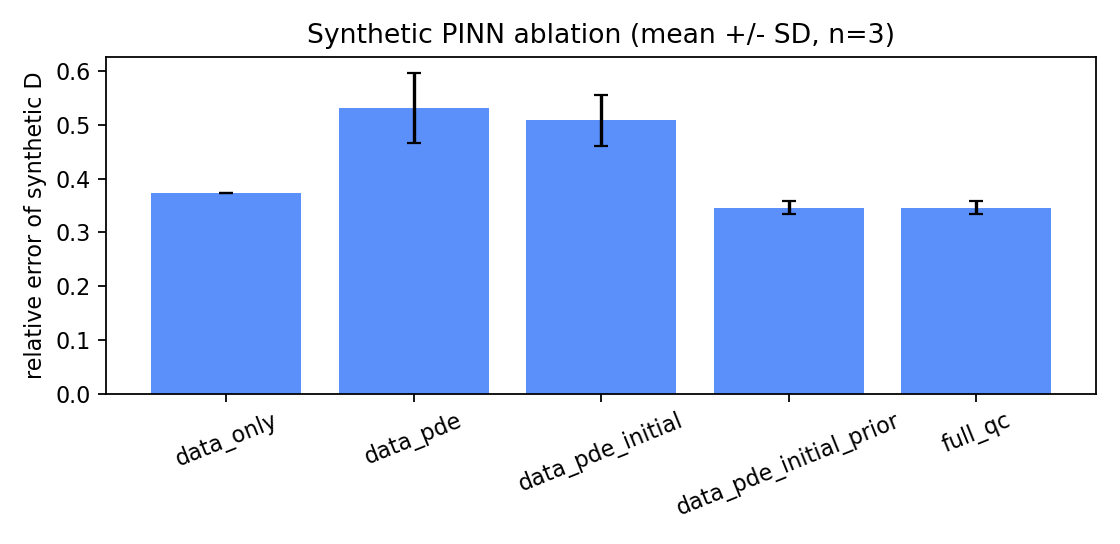
\includegraphics[width=0.78\linewidth]{../code/results/ablation_results.png}
\caption{合成PINN消融实验中$D$相对误差的均值和标准差，$n=3$。该图反映合成训练域内的优化差异，不代表人体ECS参数估计误差。\label{fig:ablation}}
\end{figure}

\subsection{ECS跨尺度数字孪生智能体：工具链与验证}
可将系统实现为ECS跨尺度数字孪生智能体：它不是复制患者大脑的确定性模型，而是维护可更新的个体观测、物理参数区间、组织先验和机制假设。输入层接收T1/FLAIR、DWI/DTI（含DTI-ALPS代理）、体液标志物及可用的病理/动物空间组学；知识层挂载ECS方程库、A$\beta$清除和AQP4相关的版本化文献库。智能体仅在以下ECS特异性白名单中调用工具：
\begin{enumerate}
\item DTI运动、涡流和协议质控工具；若质控失败，终止反演并请求重采或人工复核。
\item 基于随机游走或蒙特卡洛扩散模拟的曲折度、有效扩散敏感性分析工具，用于比较候选$\lambda$和$D^*$区间，而非从常规MRI直接宣称精确微观参数。
\item 空间组学工具（如Seurat/Squidpy工作流），用于分析AQP4相关星形胶质细胞状态、血管周围邻域与基质重塑模块\cite{satija2015,palla2022}。
\item PK/PD或对流--扩散求解器，用于研究性评估示踪剂或候选药物在假设ECS参数下的暴露分布；肿瘤药物递送场景仍须另行接受药代和安全性验证。
\item 因果图与反事实分析工具：基于预先指定的变量关系检查睡眠、年龄、血管危险因素等混杂路径，并提出最具信息量的随访或动物干预实验。
\item \textbf{主动信息增益计算与模态推荐工具}：当DTI-ALPS、CSF标志物或其他关键模态缺失时，计算候选检查在当前假设集合下预期减少的不确定性，并扣除检查风险、成本、可及性和时效性。只有净信息增益达到预设阈值且可能改变下一步决策时，才向医生提示可考虑补充的具体检查及其可区分的竞争假设；不得以追求数据完整性为由盲目推荐所有检查。
\end{enumerate}
典型流程为：先质控DTI；再调用PINN与扩散模拟模块，在明确边界条件下估计脑区$D^*$的参数区间；随后结合A$\beta$/Tau、影像及RAG证据，比对AQP4异常、基质重塑或血管因素等竞争性解释。若关键证据缺失，第六项工具给出带预期信息增益的检查建议；最后生成包含置信区间、引用定位、反证条件和后续实验的假设报告。预测、关联与因果效应仍须分别报告；智能体提供的是可计算的假设空间，而非因果结论。

\subsection{临床交互与人机协同}
临床嵌入的目标应是降低而非转移医生的认知负荷。系统宜在阅片、病历汇总或多学科讨论的既有节点提供一页式输出：以自然语言说明当前最受支持的联合表型、关键替代解释和不可回答部分；以可点击证据图谱连接原始影像区域、实验室结果、文献段落与工具日志；以置信度热力图显示哪些脑区或证据边缘受到域偏移和缺失数据影响。输出应避免冗长的模型推理文本，并把是否建议补充检查何种假设将被区分预期信息增益置于同一可审核界面。

医生保有否决、修改和延后执行建议的权利。否决必须可选择结构化原因，例如影像伪影、临床语境不符、检查禁忌或证据不足；系统将此作为审计记录，而不是自动覆盖。经伦理审批、去标识和前瞻性评估后，可将专家对建议质量、证据完整性和不当推荐的反馈用于RLHF或偏好优化，使模型学习报告措辞、停止规则和转诊边界；医疗问答中引入临床专家反馈可改善回答的对齐性，但不能替代临床效用与安全性验证\cite{singhal2023}。不得将单次医生选择当作未经验证的生物学真值。高风险输出应采用双人复核或MDT确认，并保留人工修改前后的版本。

\subsection{假设生成与Agent评估体系}
常规分类准确率不足以评估以假设生成和验证编排为目标的医疗智能体。评估应在冻结的工具版本、独立外部队列和预先注册的任务集上进行，并至少覆盖以下指标：
\begin{enumerate}
\item \textbf{证据追溯准确率（无幻觉率）}：报告中可定位至原始数据、文献或工具日志的关键主张比例，以及引用是否真实支持该主张；应由领域专家盲法核验，不以文字流畅性替代证据正确性。
\item \textbf{假设可证伪性/可验证性评分}：衡量假设是否明确给出可观测终点、竞争解释、反证条件、样本/动物分层和可执行实验Protocol。不能转化为预注册实验或无法被潜在结果推翻的陈述，应判为低分。
\item \textbf{物理一致性}：检验PINN反演参数是否违反非负性、质量守恒、边界条件、已知生理范围或稳定性约束；同时报告方程残差、后验覆盖率和对边界条件的敏感性，而非只报告拟合误差。
\item \textbf{信息增益有效性}：比较推荐检查与常规路径在真实随访中减少假设不确定性、改变恰当临床决策或避免低价值检查的比例；须将增益与成本、风险、等待时间和患者负担共同评价。
\item \textbf{人机协同性与安全性}：记录医生接受、否决和修正建议的原因，测量完成任务时间、认知负荷、关键遗漏率和不当自动化依赖；对域外、缺失模态和证据冲突病例分别报告拒答或升级人工复核的表现。
\end{enumerate}
这些指标将生成得像转化为可追溯、可反驳、受物理约束且在临床流程中有净收益的可审计要求。

\section{挑战、伦理与展望}
ECS研究的核心难题是跨尺度：微观结构、示踪动力学、宏观影像和临床结局不能简单等同。多中心协作需统一元数据、扫描协议、质控阈值和标注规范。对高风险输出，应设置域外检测、关键模态缺失拦截、人工复核队列和模型漂移监控。真实临床数据还应遵循最小必要、去标识、分级授权、加密传输和可审计访问原则。监管上，软件的预期用途、目标人群、输入边界、更新策略和临床评价计划必须清晰界定\cite{fdaaiml2021}。

未来优先事项包括建立可复用的ECS数据标准；以动物/类器官与人群队列分层验证机制假设；开展跨中心外部验证；并将可解释性从事后可视化推进到可追溯证据、失败报告和可复现分析。走向临床的必要条件不是增加更多模态或更长的自动报告，而是让UQ明确系统何时不应外推，让人在回路的工作流明确谁能否决和如何升级，以及用假设生成专属评估体系证明推荐带来可测量的净临床收益。

\section{结论}
以AD的ECS/类淋巴清除障碍为例，多模态大模型可将宏观扩散代理、A$\beta$/Tau标志物、AQP4相关微观证据及病程信息组织为可检验的联合表型；跨尺度数字孪生智能体则可进一步编排质控、物理反演、空间组学、因果图和信息增益工具，提出具有明确反证条件的机制假设。其终极价值不在于以单一或跨尺度指标给出确定性诊断，而在于构建受物理规律与临床证据约束的假设生成与验证空间。通过量化域偏移不确定性、审慎处理缺失模态并保持医生的最终判断权，建设性假设才可能逐步转化为可信的科研与临床辅助能力；这一转化仍以独立外部验证、前瞻性研究和严格数据治理为前提。

\appendix
\section{可复现代码}
本附录收录生成合成数据、训练PINN、训练ECS样式分割基线、执行消融实验和绘制结果的源文件。运行顺序为数据生成、PINN或分割演示、消融实验、结果绘制。运行环境需要Python、NumPy、PyTorch、OpenCV、Matplotlib和Pandas。代码中的字符串与注释按源文件原样保留。

\subsection{运行配置}
\lstinputlisting[language={},caption={config.yaml}]{../code/config.yaml}

\subsection{合成数据生成}
\lstinputlisting[language=Python,caption={dataset\_generator.py}]{../code/dataset_generator.py}

\subsection{PINN示踪剂反演演示}
\lstinputlisting[language=Python,caption={pinn\_ecs.py}]{../code/pinn_ecs.py}

\subsection{ECS样式分割基线}
\lstinputlisting[language=Python,caption={ecs\_net.py}]{../code/ecs_net.py}

\subsection{消融实验}
\lstinputlisting[language=Python,caption={ablation\_experiment.py}]{../code/ablation_experiment.py}

\subsection{结果绘制}
\lstinputlisting[language=Python,caption={visualization.py}]{../code/visualization.py}

\printbibliography
\end{document}